Figure \ref{fig:errors_sm} shows the distribution of roto-translation errors
(eq. (\ref{eq:rototranslation_error})) across $E$ experiments for CSM (red),
NDT (blue), and the proposed method of FSM (green).

\begin{figure}[]\centering
  % GNUPLOT: LaTeX picture with Postscript
\begingroup
  \makeatletter
  \providecommand\color[2][]{%
    \GenericError{(gnuplot) \space\space\space\@spaces}{%
      Package color not loaded in conjunction with
      terminal option `colourtext'%
    }{See the gnuplot documentation for explanation.%
    }{Either use 'blacktext' in gnuplot or load the package
      color.sty in LaTeX.}%
    \renewcommand\color[2][]{}%
  }%
  \providecommand\includegraphics[2][]{%
    \GenericError{(gnuplot) \space\space\space\@spaces}{%
      Package graphicx or graphics not loaded%
    }{See the gnuplot documentation for explanation.%
    }{The gnuplot epslatex terminal needs graphicx.sty or graphics.sty.}%
    \renewcommand\includegraphics[2][]{}%
  }%
  \providecommand\rotatebox[2]{#2}%
  \@ifundefined{ifGPcolor}{%
    \newif\ifGPcolor
    \GPcolorfalse
  }{}%
  \@ifundefined{ifGPblacktext}{%
    \newif\ifGPblacktext
    \GPblacktexttrue
  }{}%
  % define a \g@addto@macro without @ in the name:
  \let\gplgaddtomacro\g@addto@macro
  % define empty templates for all commands taking text:
  \gdef\gplfronttext{}%
  \gdef\gplfronttext{}%
  \makeatother
  \ifGPblacktext
    % no textcolor at all
    \def\colorrgb#1{}%
    \def\colorgray#1{}%
  \else
    % gray or color?
    \ifGPcolor
      \def\colorrgb#1{\color[rgb]{#1}}%
      \def\colorgray#1{\color[gray]{#1}}%
      \expandafter\def\csname LTw\endcsname{\color{white}}%
      \expandafter\def\csname LTb\endcsname{\color{black}}%
      \expandafter\def\csname LTa\endcsname{\color{black}}%
      \expandafter\def\csname LT0\endcsname{\color[rgb]{1,0,0}}%
      \expandafter\def\csname LT1\endcsname{\color[rgb]{0,1,0}}%
      \expandafter\def\csname LT2\endcsname{\color[rgb]{0,0,1}}%
      \expandafter\def\csname LT3\endcsname{\color[rgb]{1,0,1}}%
      \expandafter\def\csname LT4\endcsname{\color[rgb]{0,1,1}}%
      \expandafter\def\csname LT5\endcsname{\color[rgb]{1,1,0}}%
      \expandafter\def\csname LT6\endcsname{\color[rgb]{0,0,0}}%
      \expandafter\def\csname LT7\endcsname{\color[rgb]{1,0.3,0}}%
      \expandafter\def\csname LT8\endcsname{\color[rgb]{0.5,0.5,0.5}}%
    \else
      % gray
      \def\colorrgb#1{\color{black}}%
      \def\colorgray#1{\color[gray]{#1}}%
      \expandafter\def\csname LTw\endcsname{\color{white}}%
      \expandafter\def\csname LTb\endcsname{\color{black}}%
      \expandafter\def\csname LTa\endcsname{\color{black}}%
      \expandafter\def\csname LT0\endcsname{\color{black}}%
      \expandafter\def\csname LT1\endcsname{\color{black}}%
      \expandafter\def\csname LT2\endcsname{\color{black}}%
      \expandafter\def\csname LT3\endcsname{\color{black}}%
      \expandafter\def\csname LT4\endcsname{\color{black}}%
      \expandafter\def\csname LT5\endcsname{\color{black}}%
      \expandafter\def\csname LT6\endcsname{\color{black}}%
      \expandafter\def\csname LT7\endcsname{\color{black}}%
      \expandafter\def\csname LT8\endcsname{\color{black}}%
    \fi
  \fi
  \setlength{\unitlength}{0.0500bp}%
  \begin{picture}(5000.00,12000.00)%
    \gplgaddtomacro\gplfronttext{%
      \colorrgb{0.00,0.00,0.00}%
      \put(518,10003){\makebox(0,0)[r]{\strut{}$0.0$}}%
      \colorrgb{0.00,0.00,0.00}%
      \put(518,10186){\makebox(0,0)[r]{\strut{}$0.005$}}%
      \colorrgb{0.00,0.00,0.00}%
      \put(518,10368){\makebox(0,0)[r]{\strut{}$0.01$}}%
      \colorrgb{0.00,0.00,0.00}%
      \put(518,10551){\makebox(0,0)[r]{\strut{}$0.015$}}%
      \colorrgb{0.00,0.00,0.00}%
      \put(518,10734){\makebox(0,0)[r]{\strut{}$0.02$}}%
      \colorrgb{0.00,0.00,0.00}%
      \put(518,10916){\makebox(0,0)[r]{\strut{}$0.025$}}%
      \colorrgb{0.00,0.00,0.00}%
      \put(518,11099){\makebox(0,0)[r]{\strut{}$0.03$}}%
      \colorrgb{0.00,0.00,0.00}%
      \put(2587,11329){\makebox(0,0){\strut{}$(\overline{\delta}_{xy}, \overline{\delta}_\theta) = (0.05 \ \text{m}, 2^\circ)$}}%
      \put(2487,11729){\makebox(0,0){\strut{}Distribution of mean roto-translation errors [(m$^2$ + rad$^2$)$^{1/2}$]}}%
    }%
    \gplgaddtomacro\gplfronttext{%
    }%
    \gplgaddtomacro\gplfronttext{%
      \colorrgb{0.00,0.00,0.00}%
      \put(518,8266){\makebox(0,0)[r]{\strut{}$0.0$}}%
      \colorrgb{0.00,0.00,0.00}%
      %\put(518,8403){\makebox(0,0)[r]{\strut{}$0.005$}}%
      \colorrgb{0.00,0.00,0.00}%
      \put(518,8540){\makebox(0,0)[r]{\strut{}$0.01$}}%
      \colorrgb{0.00,0.00,0.00}%
      %\put(518,8677){\makebox(0,0)[r]{\strut{}$0.015$}}%
      \colorrgb{0.00,0.00,0.00}%
      \put(518,8814){\makebox(0,0)[r]{\strut{}$0.02$}}%
      \colorrgb{0.00,0.00,0.00}%
      %\put(518,8951){\makebox(0,0)[r]{\strut{}$0.025$}}%
      \colorrgb{0.00,0.00,0.00}%
      \put(518,9088){\makebox(0,0)[r]{\strut{}$0.03$}}%
      \colorrgb{0.00,0.00,0.00}%
      %\put(518,9225){\makebox(0,0)[r]{\strut{}$0.035$}}%
      \colorrgb{0.00,0.00,0.00}%
      \put(518,9362){\makebox(0,0)[r]{\strut{}$0.04$}}%
      \colorrgb{0.00,0.00,0.00}%
      \put(2587,9592){\makebox(0,0){\strut{}$(\overline{\delta}_{xy}, \overline{\delta}_\theta) = (0.10 \ \text{m}, 4^\circ)$}}%
    }%
    \gplgaddtomacro\gplfronttext{%
    }%
    \gplgaddtomacro\gplfronttext{%
      \colorrgb{0.00,0.00,0.00}%
      \put(518,6530){\makebox(0,0)[r]{\strut{}$0.0$}}%
      \colorrgb{0.00,0.00,0.00}%
      \put(518,6749){\makebox(0,0)[r]{\strut{}$0.01$}}%
      \colorrgb{0.00,0.00,0.00}%
      \put(518,6968){\makebox(0,0)[r]{\strut{}$0.02$}}%
      \colorrgb{0.00,0.00,0.00}%
      \put(518,7188){\makebox(0,0)[r]{\strut{}$0.03$}}%
      \colorrgb{0.00,0.00,0.00}%
      \put(518,7407){\makebox(0,0)[r]{\strut{}$0.04$}}%
      \colorrgb{0.00,0.00,0.00}%
      \put(518,7626){\makebox(0,0)[r]{\strut{}$0.05$}}%
      \colorrgb{0.00,0.00,0.00}%
      \put(2587,7856){\makebox(0,0){\strut{}$(\overline{\delta}_{xy}, \overline{\delta}_\theta) = (0.15 \ \text{m}, 8.6^\circ)$}}%
    }%
    \gplgaddtomacro\gplfronttext{%
    }%
    \gplgaddtomacro\gplfronttext{%
      \colorrgb{0.00,0.00,0.00}%
      \put(518,4793){\makebox(0,0)[r]{\strut{}$0.0$}}%
      \colorrgb{0.00,0.00,0.00}%
      \put(518,4976){\makebox(0,0)[r]{\strut{}$0.01$}}%
      \colorrgb{0.00,0.00,0.00}%
      \put(518,5158){\makebox(0,0)[r]{\strut{}$0.02$}}%
      \colorrgb{0.00,0.00,0.00}%
      \put(518,5341){\makebox(0,0)[r]{\strut{}$0.03$}}%
      \colorrgb{0.00,0.00,0.00}%
      \put(518,5524){\makebox(0,0)[r]{\strut{}$0.04$}}%
      \colorrgb{0.00,0.00,0.00}%
      \put(518,5706){\makebox(0,0)[r]{\strut{}$0.05$}}%
      \colorrgb{0.00,0.00,0.00}%
      \put(518,5889){\makebox(0,0)[r]{\strut{}$0.06$}}%
      \colorrgb{0.00,0.00,0.00}%
      \put(2587,6119){\makebox(0,0){\strut{}$(\overline{\delta}_{xy}, \overline{\delta}_\theta) = (0.20 \ \text{m}, 17.2^\circ)$}}%
    }%
    \gplgaddtomacro\gplfronttext{%
    }%
    \gplgaddtomacro\gplfronttext{%
      \colorrgb{0.00,0.00,0.00}%
      \put(518,3056){\makebox(0,0)[r]{\strut{}$0.0$}}%
      \colorrgb{0.00,0.00,0.00}%
      \put(518,3275){\makebox(0,0)[r]{\strut{}$0.02$}}%
      \colorrgb{0.00,0.00,0.00}%
      \put(518,3494){\makebox(0,0)[r]{\strut{}$0.04$}}%
      \colorrgb{0.00,0.00,0.00}%
      \put(518,3714){\makebox(0,0)[r]{\strut{}$0.06$}}%
      \colorrgb{0.00,0.00,0.00}%
      \put(518,3933){\makebox(0,0)[r]{\strut{}$0.08$}}%
      \colorrgb{0.00,0.00,0.00}%
      \put(518,4152){\makebox(0,0)[r]{\strut{}$0.10$}}%
      \colorrgb{0.00,0.00,0.00}%
      \put(2587,4382){\makebox(0,0){\strut{}$(\overline{\delta}_{xy}, \overline{\delta}_\theta) = (0.20 \ \text{m}, 32^\circ)$}}%
    }%
    \gplgaddtomacro\gplfronttext{%
    }%
    \gplgaddtomacro\gplfronttext{%
      \colorrgb{0.00,0.00,0.00}%
      \put(518,1320){\makebox(0,0)[r]{\strut{}$0.0$}}%
      \colorrgb{0.00,0.00,0.00}%
      \put(518,1594){\makebox(0,0)[r]{\strut{}$0.05$}}%
      \colorrgb{0.00,0.00,0.00}%
      \put(518,1868){\makebox(0,0)[r]{\strut{}$0.10$}}%
      \colorrgb{0.00,0.00,0.00}%
      \put(518,2142){\makebox(0,0)[r]{\strut{}$0.15$}}%
      \colorrgb{0.00,0.00,0.00}%
      \put(518,2416){\makebox(0,0)[r]{\strut{}$0.20$}}%
      \colorrgb{0.00,0.00,0.00}%
      \put(1037,1100){\makebox(0,0){\strut{}$0.0$}}%
      \colorrgb{0.00,0.00,0.00}%
      \put(1812,1100){\makebox(0,0){\strut{}$0.01$}}%
      \colorrgb{0.00,0.00,0.00}%
      \put(2587,1100){\makebox(0,0){\strut{}$0.03$}}%
      \colorrgb{0.00,0.00,0.00}%
      \put(3362,1100){\makebox(0,0){\strut{}$0.05$}}%
      \colorrgb{0.00,0.00,0.00}%
      \put(4137,1100){\makebox(0,0){\strut{}$0.10$}}%
      \colorrgb{0.00,0.00,0.00}%
      \put(2587,770){\makebox(0,0){\strut{}sd of sensor measurement noise $\sigma_R$ [m]}}%
      \colorrgb{0.00,0.00,0.00}%
      \put(2587,2646){\makebox(0,0){\strut{}$(\overline{\delta}_{xy}, \overline{\delta}_\theta) = (0.20 \ \text{m}, 45^\circ)$}}%
    }%
    \put(0,0){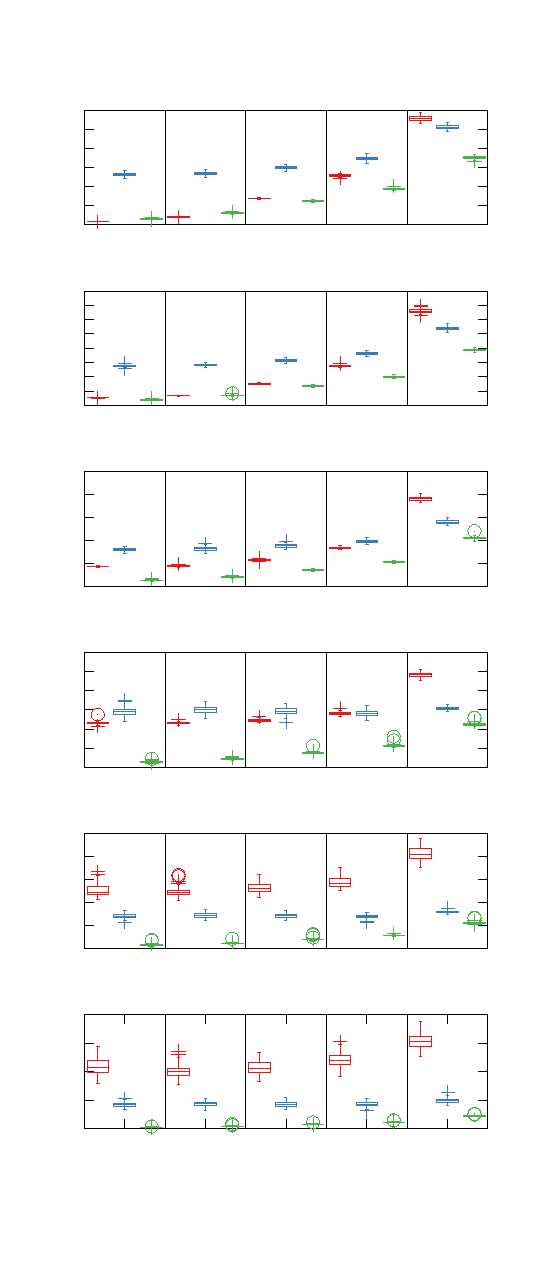
\includegraphics{./figures/experiments/errors_CSM_NDT_implm6_short}}%
    \gplfronttext
  \end{picture}%
\endgroup

  \caption{\small Distribution of mean errors of CSM (red), NDT (blue), and
           FSM (our approach) across a range of maximal positional and
           orientational displacements, for progressively larger sensor
           measurement noise levels. The variability of FSM's rigid body
           transformation error is consistent across all configurations. The
           error is independent of the initial displacement of scans for a
           given level of sensor noise}
  \label{fig:errors_sm}
\end{figure}

At small location and orientation displacements between the two input scans
($\overline{\delta}_{xy} \leq $ 0.05 m,
$\overline{\delta}_\theta \leq 2^\circ$), CSM outperforms NDT and FSM for low
levels of sensor noise ($\sigma_R \leq 0.01$ m). However, as noise increases,
FSM starts exhibiting greater robustness and accuracy than CSM. At
greater location and orientation displacements
($\overline{\delta}_{xy} > 0.05$ m,
$\overline{\delta}_\theta > 2^\circ$), FSM is able to maintain errors equal to
or lower than CSM across the entirety of the spectrum of tested noise levels.
Compared to the equally correspondenceless method of NDT, FSM exhibits greater
accuracy across all tested configurations. The variability of FSM's errors
for a given level of sensor noise is independent of the displacement of the
two input scans. The juxtaposition of the three methods' pose errors at high
levels of sensor noise highlight the robustness afforded to FSM by the Discrete
Fourier transform and its properties. In terms of execution time, CSM ranged
from $4.8$ to $20.5$ ms, NDT from $8.1$ to $19.9$ ms, and FSM from $13.2$ to
$16.7$ ms. Therefore FSM's exhibits the least variability to sensor noise and
locational and orientational displacement in terms of runtime. The measurement
frequency of modern LIDAR sensors ranges from $12$-$20$ Hz; therefore FSM runs
in real time in modern processors.
